% !TEX root = ./notes.tex
\section{Experiments}
In our experiments, we use the Penn Treebank corpus (PTB) \citep{marcus1993building}, and the Wikitext-2 dataset \citep{merity2016pointer}.
PTB has been a standard dataset used for benchmarking language models.
It consists of $923$k training, $73$k validation, and $82$k test words.
The version of this dataset which we use is the one processed in \citet{mikolov2010recurrent}, with the most frequent $10$k words selected to be in the vocabulary and rest replaced with a an $<$unk$>$ token \footnote{PTB can be downloaded at \href{url}{http://www.fit.vutbr.cz/~imikolov/rnnlm/simple-examples.tgz}}.
Wikitext-2 is a dataset released recently as an alternative to PTB\footnote{Wikitext-2 can be downloaded at \href{url}{https://s3.amazonaws.com/research.metamind.io/wikitext/wikitext-2-v1.zip}}.
It contains $2,088$k training, $217$k validation, and $245$k test tokens, and has a vocabulary of $33,278$ words; therefore, in comparison to PTB, it is roughly 2 times larger in dataset size, and 3 times larger in vocabulary.

\subsection{Model and Training Highlights}
We closely follow the LSTM based language model proposed in \citet{zaremba2014recurrent} for constructing our baseline model. 
Specifically, we use a $2$-layer LSTM with the same number of hidden units in each layer, and we use $3$ different network sizes: small ($200$ units), medium ($650$ units), and large ($1500$ units).
We train our models using stochastic gradient descent, and we use a variant of the dropout method proposed in \citet{gal2015theoretically}.
We defer further details regarding training the models to section \ref{section:Train-details} of the appendix.
We refer to our baseline network as variational dropout LSTM, or VD-LSTM in short.
%The codebase for reproducing our results is going to be made public in the near future.

\subsection{Empirical Validation for the Theory of Reusing Word Embeddings}
In Section \ref{section:RE}, we showed that the particular loss augmentation scheme we choose constrains the output projection matrix to be close to the input embedding matrix, without explicitly doing so by reusing the input embedding matrix.
As a first experiment, we set out to validate this theoretical result.
To do this, we try to simulate the setting in Section \ref{section:RE} by doing the following: We select a randomly chosen $20,000$ contiguous word sequence in the PTB training set, and train a 2-layer LSTM language model with 300 units in each layer with loss augmentation by minimizing the following loss:
\eq{
\label{eqn:AL_mixture}
J^{tot} = \beta \Jaug \tau^2|V| + (1-\beta)J.
}
Here, $\beta$ is the proportion of the augmented loss used in the total loss, and $\Jaug$ is scaled by $\tau^2|V|$ to approximately match the magnitudes of the derivatives of $J$ and $\Jaug$ (see \eqref{eqn:Jaug_matching_logits}).
Since we aim to achieve the minimum training loss possible, and the goal is to show a particular result rather than to achieve good generalization, we do not use any kind of regularization in the neural network (e.g. weight decay, dropout).
For this set of experiments, we also constrain each row of the input embedding matrix to have a norm of $1$ because training becomes difficult without this constraint when only augmented loss is used.
After training, we compute a metric that measures distance between the subspace spanned by the rows of the input embedding matrix, $L$, and that spanned by the columns of the output projection matrix, $W$. For this, we use a common metric based on the relative residual norm from projection of one matrix onto another \citep{bjorck1973numerical}.
The computed distance between the subspaces is $1$ when they are orthogonal, and $0$ when they are the same.
Interested reader may refer to section \ref{section:subspace-dist} in the appendix for the details of this metric.

Figure \ref{fig:normdist} shows the results from two tests. In one (panel a), we test the effect of using the augmented loss by sweeping $\beta$ in \eqref{eqn:AL_mixture} from $0$ to $1$ at a reasonably high temperature ($\tau=10$).
With no loss augmentation ($\beta=0$), the distance is almost $1$, and as more and more augmented loss is used the distance decreases rapidly, and eventually reaches around $0.06$ when only augmented loss is used.
In the second test (panel b), we set $\beta=1$, and try to see the effect of the temperature on the subspace distance (remember the theory predicts low distance when $\tau \rightarrow \infty$).
Notably, the augmented loss causes $W$ to approach $L^T$ sufficiently even at temperatures as low as $2$, although higher temperatures still lead to smaller subspace distances.

\begin{figure*}[t!]
    \centering
    \begin{subfigure}[t]{0.5\textwidth}
        \centering
        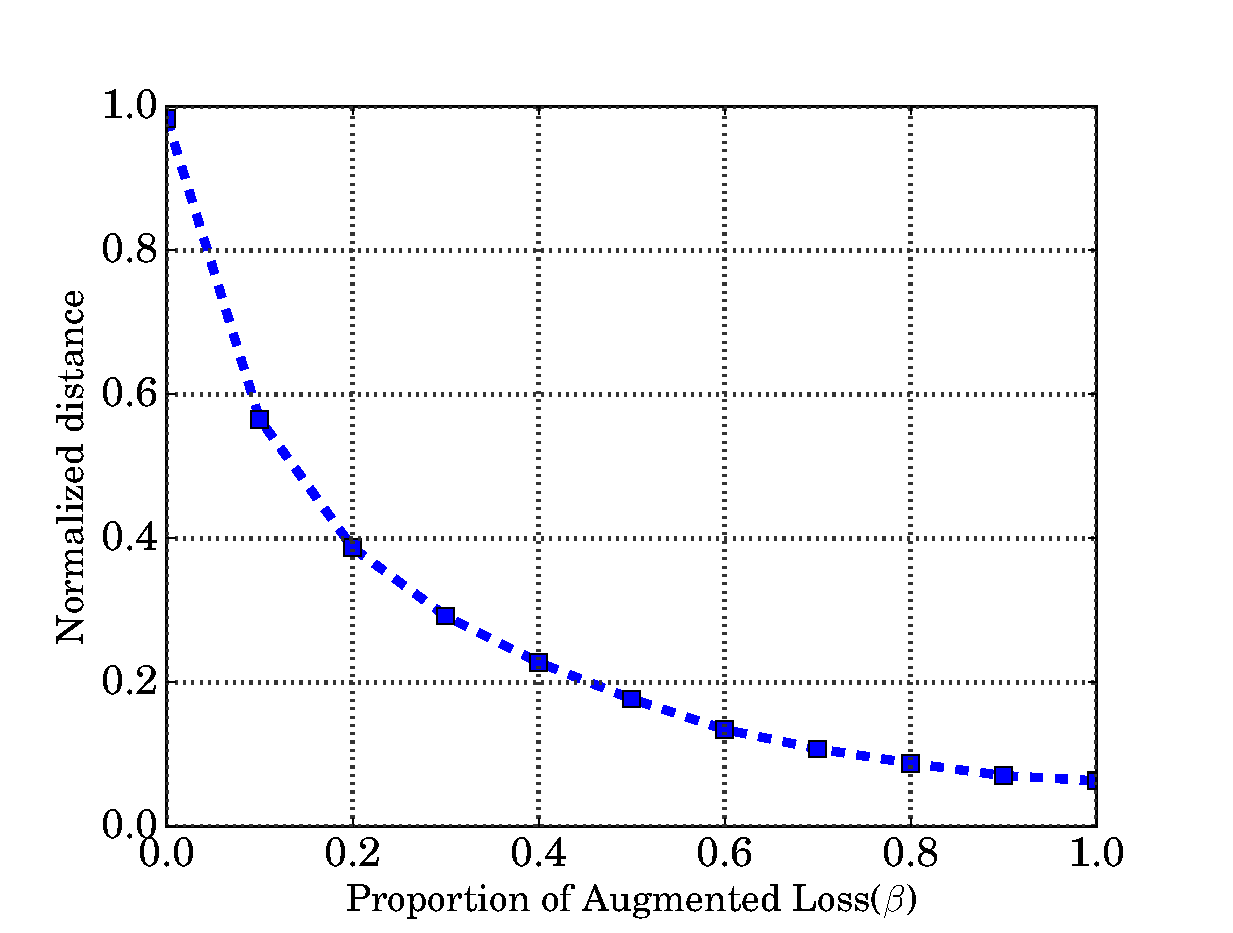
\includegraphics[scale=0.32]{Prop.eps}
        \caption{Subspace distance at $\tau=10$ for \\ different proportions of $\Jaug$}
    \end{subfigure}%
    ~ 
    \begin{subfigure}[t]{0.5\textwidth}
        \centering
        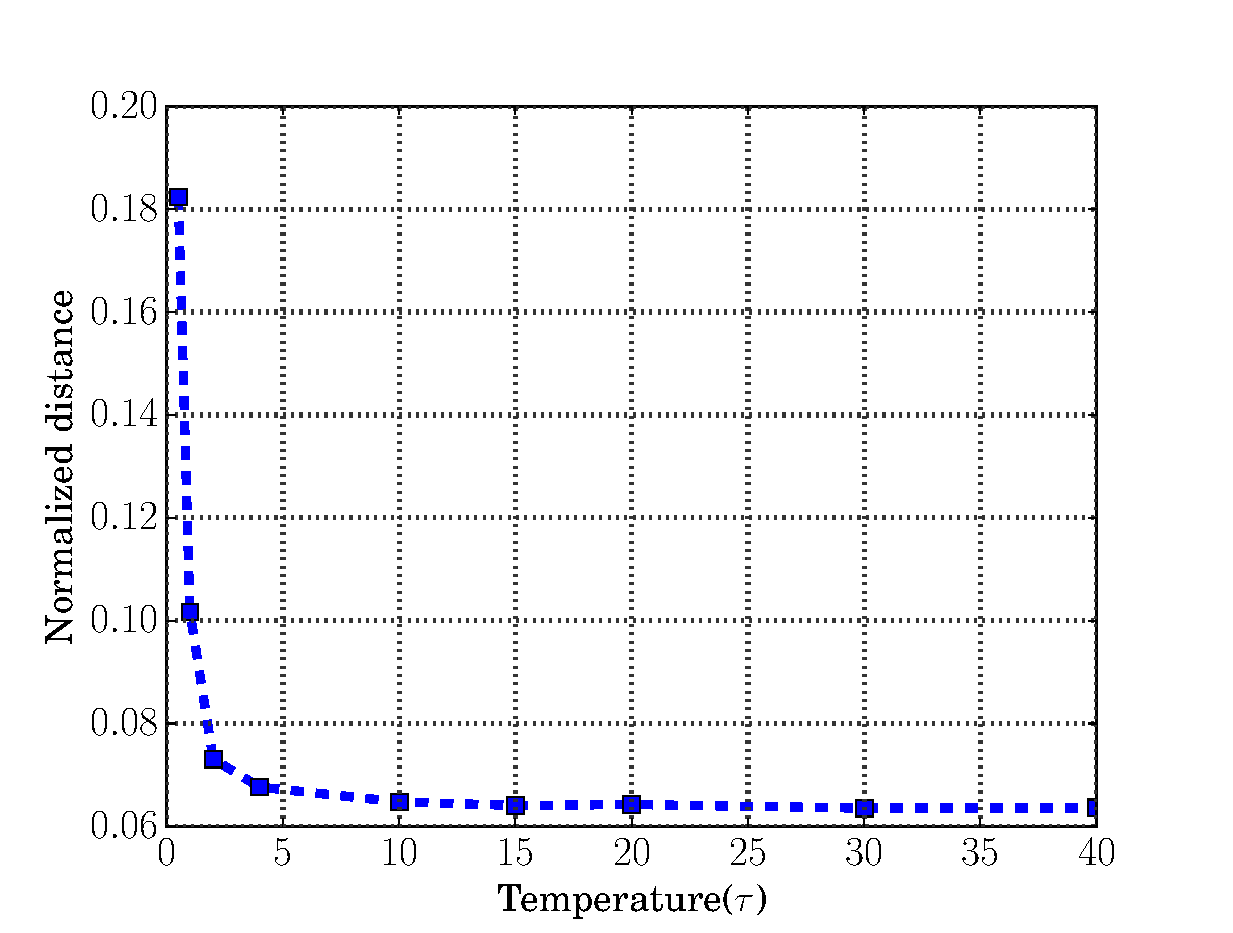
\includegraphics[scale=0.32]{Temp.eps}
        \caption{Subspace distance at different temp-\\eratures  when only $\Jaug$ is used}
    \end{subfigure}
    \caption{Subspace distance between $L^T$ and $W$ for different experiment conditions for the validation experiments. Results are averaged over $10$ independent runs. These results validate our theory under practical conditions.}
    \label{fig:normdist}
\end{figure*}

These results confirm the mechanism through which our proposed loss pushes $W$ to learn the same column space as $L^T$, and it suggests that reusing the input embedding matrix by explicitly constraining $W=L^T$ is not simply a kind of regularization, but is in fact an optimal choice in our framework.
What can be achieved separately with each of the two proposed improvements as well as with the two of them combined is a question of empirical nature, which we investigate in the next section.

\subsection{Results on PTB and Wikitext-2 Datasets}
In order to investigate the extent to which each of our proposed improvements helps with learning, we train 4 different models for each network size:
(1) 2-Layer LSTM with variational dropout (VD-LSTM)
(2) 2-Layer LSTM with variational dropout and augmented loss (VD-LSTM +AL)
(3) 2-Layer LSTM with variational dropout and reused embeddings (VD-LSTM +RE)
(4) 2-Layer LSTM with variational dropout and both RE and AL (VD-LSTM +REAL).

Figure \ref{fig:val_perp_4models} shows the validation perplexities of the four models during training on the PTB corpus for small (panel a) and large (panel b) networks. All of AL, RE, and REAL networks significantly outperform the baseline in both cases.
Table \ref{table:comp-our} compares the final validation and test perplexities of the four models on both PTB and Wikitext-2 for each network size.
In both datasets, both AL and RE improve upon the baseline individually, and using RE and AL together leads to the best performance.
Based on performance comparisons, we make the following notes on the two proposed improvements:
\begin{itemize}[noitemsep]
\item AL provides better performance gains for smaller networks.
This is not surprising given the fact that small models are rather inflexible, and one would expect to see improved learning by training against a more informative data distribution (contributed by the augmented loss) (see \citet{hinton2015distilling}). 
For the smaller PTB dataset, performance with AL surpasses that with RE. In comparison, for the larger Wikitext-2 dataset, improvement by AL is more limited. 
This is expected given larger training sets better represent the true data distribution, mitigating the supervision problem.
In fact, we set out to validate this reasoning in a direct manner, and additionally train the small networks separately on the first and second halves of the Wikitext-2 training set.
This results in two distinct datasets which are each about the same size as PTB (1044K vs 929K).
As can be seen in Table \ref{table:wiki-valid}, AL has significantly improved competitive performance against RE and REAL despite the fact that embedding size is 3 times larger compared to PTB.
These results support our argument that the proposed augmented loss term acts to improve the amount of information gathered from the dataset.
\item RE significantly outperforms AL for larger networks.
This indicates that, for large models, the more effective mechanism of our proposed framework is the one which enforces proximity between the output projection space and the input embedding space.
From a model complexity perspective, the nontrivial gains offered by RE for all network sizes and for both datasets could be largely attributed to its explicit function to reduce the model size while preserving the representational power according to our framework.
%The fact that RE offers nontrivial gains for any model size for both datasets is also due to its explicit function to reduce the model size while preserving the representational power according to our framework.
\end{itemize}

We list in Table \ref{table-benchmark} the comparison of models with and without our proposed modifications on the Penn Treebank Corpus. The best LSTM model (VD-LSTM+REAL) outperforms all previous work which uses conventional framework, including large ensembles. The recently proposed recurrent highway networks \citep{zilly2016recurrent} when trained with reused embeddings (VD-RHN +RE) achieves the best overall performance, improving on VD-RHN by a perplexity of $2.5$.

\begin{figure*}[t!]
    \centering
    \begin{subfigure}[t]{0.5\textwidth}
        \centering
        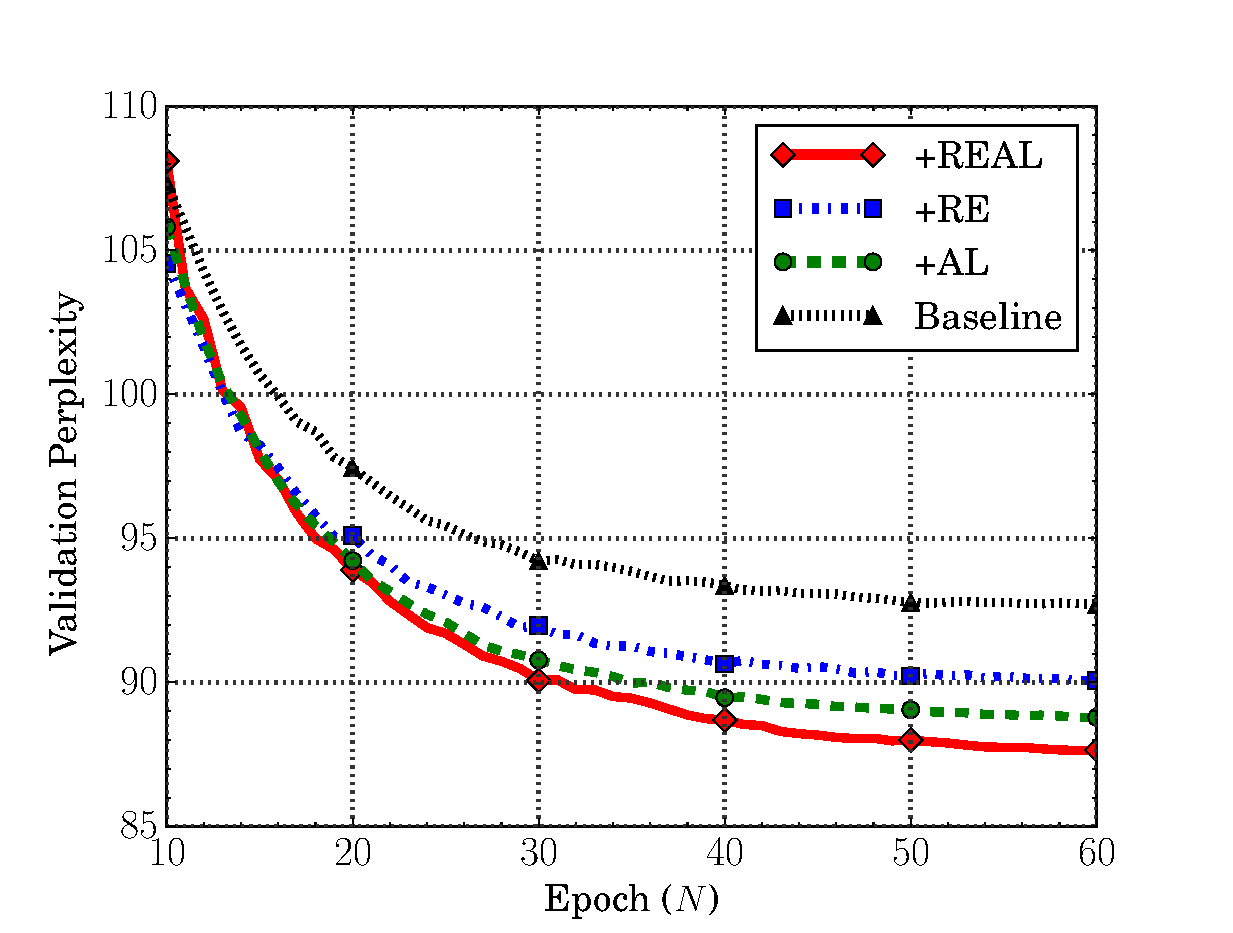
\includegraphics[scale=0.32]{REAL_Small_valid_new_notscaled.eps}
        \caption{Small Network}
    \end{subfigure}%
    ~ 
    \begin{subfigure}[t]{0.5\textwidth}
        \centering
        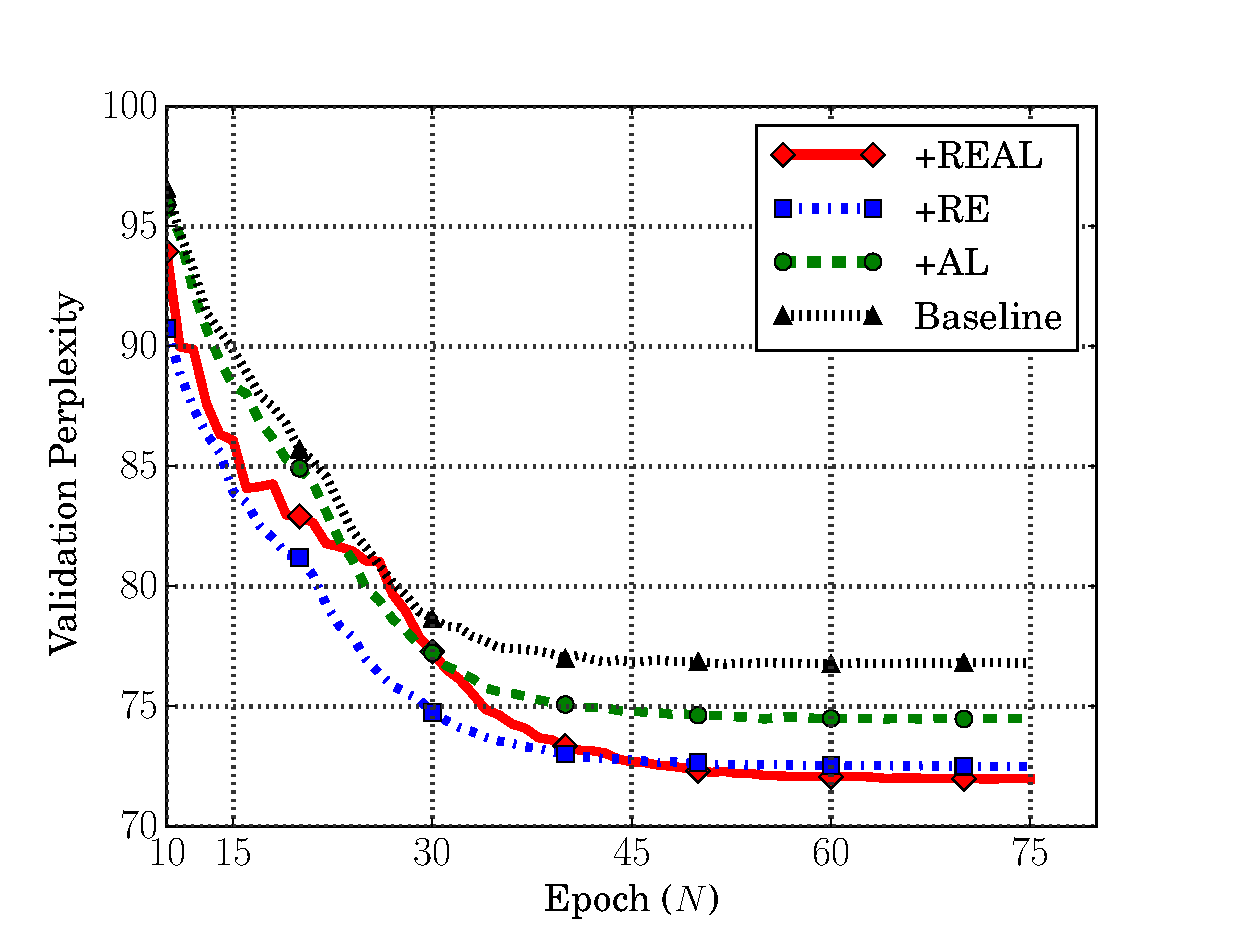
\includegraphics[scale=0.32]{REAL_Large_valid_notscaled.eps}
        \caption{Large Network}
    \end{subfigure}
    \caption{Progress of validation perplexities during training for the $4$ different models for two (small ($200$) and large ($1500$)) network sizes.}
    \label{fig:val_perp_4models}
\end{figure*}



\begin{table}[ht]\footnotesize
\caption{Comparison of the final word level perplexities on the validation and test set for the $4$ different models.}
\label{table:comp-our}
\begin{center}
{\def\arraystretch{1.2}
 \begin{tabular}{c | l c c @{\hskip 10mm} c c} 
 \multicolumn{2}{c}{} & \multicolumn{2}{c}{ \bf PTB \hspace{5mm} } & \multicolumn{2}{c}{\bf Wikitext-2 \hspace{2mm} } \\  
\bf Network & \bf Model \hspace{5mm} & \bf Valid & \bf Test  &  \bf Valid & \bf Test \\
\hline 
\multirow{4}{4em}{Small\tablefootnote{For PTB, small models were re-trained by initializing to their final configuration from the first training session. This did not change the final perplexity for baseline, but lead to improvements for the other models.}  \\ (200 units)}
 & VD-LSTM & 92.6 & 87.3 & 112.2 & 105.9\\ 
 & VD-LSTM+AL& 86.3 & 82.9 & 110.3 & 103.8  \\ 
 & VD-LSTM+RE & 89.9 & 85.1 & 106.1 & 100.5 \\
 & VD-LSTM+REAL & 86.3 & 82.7 & 105.6 & 98.9\\ 
 \hline 
 \multirow{4}{4em}{Medium \\ (650 units)} 
 & VD-LSTM & 82.0 & 77.7 & 100.2 & 95.3 \\ 
 & VD-LSTM+AL & 77.4 & 74.7 & 98.8 & 93.1 \\ 
 & VD-LSTM+RE & 77.1 & 73.9  & 92.3 & 87.7\\
 & VD-LSTM+REAL & 75.7 & 73.2 & 91.5 & 87.0\\ 
 \hline
 \multirow{4}{4em}{Large\tablefootnote{Large network results on Wikitext-2 are not reported since computational resources were insufficient to run some of the configurations.} \\ (1500 units)} 
 & VD-LSTM & 76.8 & 72.6 & - & -\\ 
 & VD-LSTM+AL & 74.5 & 71.2 & - & - \\ 
 & VD-LSTM+RE & 72.5 & 69.0 & - & - \\
 & VD-LSTM+REAL & 71.1 & 68.5 & - & -\\
 \hline
\end{tabular}
}
\end{center}
\end{table}

\begin{table}[ht]\footnotesize
\caption{Performance of the four different small models trained on the equally sized two partitions of Wikitext-2 training set. These results are consistent with those on PTB (see Table \ref{table:comp-our}), which has a similar training set size with each of these partitions, although its word embedding dimension is three times smaller. }
\label{table:wiki-valid}
\begin{center}
{\def\arraystretch{1.2}
 \begin{tabular}{c | l c c c c} 
 \multicolumn{2}{c}{} & \multicolumn{2}{c}{\bf Wikitext-2, Partition 1} & \multicolumn{2}{c}{\bf Wikitext-2, Partition 2} \\  
\bf Network & \bf Model \hspace{5mm} & \bf Valid & \bf Test  & \bf Valid & \bf Test \\
\hline 
\multirow{4}{4em}{Small  \\ (200 units)}
 & VD-LSTM & 159.1 & 148.0 & 163.19 & 148.6\\ 
 & VD-LSTM+AL& 153.0 & 142.5 & 156.4 & 143.7  \\ 
 & VD-LSTM+RE & 152.4 & 141.9 & 152.5 & 140.9 \\
 & VD-LSTM+REAL & 149.3 & 140.6 & 150.5 & 138.4\\ 
 \hline 
\end{tabular}
}
\end{center}
\end{table}

\begin{table}[htbp]\footnotesize
\caption{Comparison of our work to previous state of the art on word-level validation and test perplexities  on the Penn Treebank corpus. Models using our framework significantly outperform other models.}
\label{table-benchmark}
\begin{center}
{\def\arraystretch{1.2}
 \begin{tabular}{l | c c c} 
\bf Model & \bf Parameters & \bf Validation & \bf Test \\ 
\hline 
 RNN \citep{mikolov2012context}  & 6M & - & 124.7 \\
 RNN+LDA \citep{mikolov2012context} & 7M & - & 113.7 \\ 
 RNN+LDA+KN-5+Cache \citep{mikolov2012context} & 9M & - & 92.0 \\ 
 Deep RNN \citep{PascanuGCB13} & 6M & - & 107.5 \\
Sum-Prod Net \citep{cheng2014language} & 5M & - & 100.0 \\
LSTM (medium) \citep{zaremba2014recurrent} & 20M & 86.2 & 82.7 \\
CharCNN \citep{kim2015character} & 19M & - & 78.9 \\
LSTM (large) \citep{zaremba2014recurrent} & 66M & 82.2 & 78.4 \\
VD-LSTM (large, untied, MC) \citep{gal2015theoretically} & 66M & - & $73.4 \pm 0.0$ \\
Pointer Sentinel-LSTM(medium) \citep{merity2016pointer} & 21M & 72.4 & 70.9 \\
38 Large LSTMs \citep{zaremba2014recurrent} & 2.51B & 71.9 & 68.7 \\
10 Large VD-LSTMs \citep{gal2015theoretically} & 660M & - & 68.7 \\
VD-RHN \citep{zilly2016recurrent} & 32M & 71.2 & 68.5 \\
 \hline
VD-LSTM +REAL (large) & 51M & 71.1 & 68.5 \\
VD-RHN +RE \citep{zilly2016recurrent} \tablefootnote{This model was developed following our work in \citet{inanimproved}.} & 24M & \bf{68.1} & \bf{66.0} \\
 \hline
\end{tabular}
}
\end{center}
\end{table}


\subsection{Qualitative Results}
One important feature of our framework that leads to better word predictions is the explicit mechanism to assign probabilities to words not merely according to the observed output statistics, but also considering the metric similarity between words.
We observe direct consequences of this mechanism qualitatively in the Penn Treebank in different ways: First, we notice that the probability of generating the $<$unk$>$ token with our proposed network (VD-LSTM +REAL) is significantly lower compared to the baseline network (VD-LSTM) across many words.
This could be explained by noting the fact that the $<$unk$>$ token is an aggregated token rather than a specific word, and it is often not expected to be close to specific words in the word embedding space.
We observe the same behavior with very frequent words such as "a", "an", and "the", owing to the same fact that they are not correlated with particular words.
Second, we not only observe better probability assignments for the target words, but we also observe relatively higher probability weights associated with the words close to the targets.
Sometimes this happens in the form of predicting words semantically close together which are plausible even when the target word is not successfully captured by the model.
We provide a few examples from the PTB test set which compare the prediction performance of $1500$ unit VD-LSTM and $1500$ unit VD-LSTM +REAL in table \ref{table:qualitative}.
We would like to note that prediction performance of VD-LSTM +RE is similar to VD-LSTM +REAL for the large network.

\begin{table}[h]\footnotesize
\caption{Prediction for the next word by the baseline (VD-LSTM) and proposed (VD-LSTM +REAL) networks for a few example phrases in the PTB test set. Top $10$ word predictions are sorted in descending probability, and are arranged in column-major format.}
\label{table:qualitative}
\begin{center}
{\def\arraystretch{1.2}
 \begin{tabular}{l | l l l}
\textbf{Phrase} + \emph{Next word(s)} & \bf \begin{tabular}{@{}c@{}}Top 10 predicted words \\ VD-LSTM\end{tabular} & \bf \begin{tabular}{@{}c@{}}Top 10 predicted words \\ VD-LSTM +REAL\end{tabular} \\ 
\hline
\begin{tabular}{l}information international \\ said it believes that  the \\ complaints filed in \\ + \emph{federal court} \end{tabular}   &  
\begin{tabular}{l l}the 0.27 & an 0.03 \\ a 0.13 & august 0.01\\ \bf federal 0.13  & new 0.01\\ N 0.09 &response 0.01\\ $\<$unk$\>$ 0.05 & connection 0.01   \end{tabular}  & 
\begin{tabular}{l l}\bf federal 0.22 & connection 0.03 \\ the 0.1 & august 0.03\\ a 0.08  & july 0.03\\ N 0.06 &an 0.03\\ state 0.04 & september 0.03   \end{tabular} \\
 \hline 
\begin{tabular}{l}oil company refineries \\ ran flat out to prepare \\ for a robust holiday \\ driving season in july and \\ + \emph{august}\end{tabular} & 
\begin{tabular}{l l}the 0.09 & in 0.03 \\ N 0.08 & has 0.03\\ a 0.07  & is 0.02\\ $\<$unk$\>$ 0.07 &will 0.02\\ was 0.04 & its 0.02   \end{tabular}  & 
\begin{tabular}{l l}\bf august 0.08 & a 0.03 \\ N 0.05 & in 0.03\\ early 0.05  & that 0.02\\ september 0.05 &ended 0.02\\ the 0.03 & its 0.02   \end{tabular} \\
 \hline
\begin{tabular}{l}southmark said it plans \\ to $\<$unk$\>$ its $\<$unk$\>$ to \\ provide financial results \\ as soon as its audit is \\ + \emph{completed}\end{tabular} & 
\begin{tabular}{l l}the 0.06 & to 0.03 \\ $\<$unk$\>$ 0.05 & likely 0.03\\ a 0.05  & expected 0.03\\ in 0.04 & scheduled 0.01\\ n't 0.04 & \bf completed 0.01   \end{tabular}  & 
\begin{tabular}{l l}expected 0.1 & a 0.03 \\ \bf completed 0.04 & scheduled 0.03\\ $\<$unk$\>$ 0.03  & n't 0.03\\ the 0.03 &due 0.02\\ in 0.03 & to 0.01   \end{tabular} \\
 \hline
 \begin{tabular}{l}merieux said the \\ government 's minister \\ of industry science and \\ + \emph{technology}\end{tabular} & 
\begin{tabular}{l l}$\<$unk$\>$ 0.33 & industry 0.01 \\ the 0.06 & commerce 0.01\\ a 0.01  & planning 0.01\\ other 0.01 & management 0.01\\ others 0.01 & mail 0.01  \end{tabular}  & 
\begin{tabular}{l l}$\<$unk$\>$ 0.09 & industry 0.03 \\ health 0.08 & business 0.02\\ development 0.04  & telecomm. 0.02\\ the 0.04 &human 0.02\\ a 0.03 & other 0.01   \end{tabular} \\
\hline
\end{tabular}
}
\end{center}
\end{table}
